\documentclass[twoside]{book}

% Packages required by doxygen
\usepackage{fixltx2e}
\usepackage{calc}
\usepackage{doxygen}
\usepackage{graphicx}
\usepackage[utf8]{inputenc}
\usepackage{makeidx}
\usepackage{multicol}
\usepackage{multirow}
\PassOptionsToPackage{warn}{textcomp}
\usepackage{textcomp}
\usepackage[nointegrals]{wasysym}
\usepackage[table]{xcolor}

% Font selection
\usepackage[T1]{fontenc}
\usepackage{mathptmx}
\usepackage[scaled=.90]{helvet}
\usepackage{courier}
\usepackage{amssymb}
\usepackage{sectsty}
\renewcommand{\familydefault}{\sfdefault}
\allsectionsfont{%
  \fontseries{bc}\selectfont%
  \color{darkgray}%
}
\renewcommand{\DoxyLabelFont}{%
  \fontseries{bc}\selectfont%
  \color{darkgray}%
}
\newcommand{\+}{\discretionary{\mbox{\scriptsize$\hookleftarrow$}}{}{}}

% Page & text layout
\usepackage{geometry}
\geometry{%
  a4paper,%
  top=2.5cm,%
  bottom=2.5cm,%
  left=2.5cm,%
  right=2.5cm%
}
\tolerance=750
\hfuzz=15pt
\hbadness=750
\setlength{\emergencystretch}{15pt}
\setlength{\parindent}{0cm}
\setlength{\parskip}{0.2cm}
\makeatletter
\renewcommand{\paragraph}{%
  \@startsection{paragraph}{4}{0ex}{-1.0ex}{1.0ex}{%
    \normalfont\normalsize\bfseries\SS@parafont%
  }%
}
\renewcommand{\subparagraph}{%
  \@startsection{subparagraph}{5}{0ex}{-1.0ex}{1.0ex}{%
    \normalfont\normalsize\bfseries\SS@subparafont%
  }%
}
\makeatother

% Headers & footers
\usepackage{fancyhdr}
\pagestyle{fancyplain}
\fancyhead[LE]{\fancyplain{}{\bfseries\thepage}}
\fancyhead[CE]{\fancyplain{}{}}
\fancyhead[RE]{\fancyplain{}{\bfseries\leftmark}}
\fancyhead[LO]{\fancyplain{}{\bfseries\rightmark}}
\fancyhead[CO]{\fancyplain{}{}}
\fancyhead[RO]{\fancyplain{}{\bfseries\thepage}}
\fancyfoot[LE]{\fancyplain{}{}}
\fancyfoot[CE]{\fancyplain{}{}}
\fancyfoot[RE]{\fancyplain{}{\bfseries\scriptsize Generated on Thu Oct 20 2016 09\+:32\+:25 for My Project by Doxygen }}
\fancyfoot[LO]{\fancyplain{}{\bfseries\scriptsize Generated on Thu Oct 20 2016 09\+:32\+:25 for My Project by Doxygen }}
\fancyfoot[CO]{\fancyplain{}{}}
\fancyfoot[RO]{\fancyplain{}{}}
\renewcommand{\footrulewidth}{0.4pt}
\renewcommand{\chaptermark}[1]{%
  \markboth{#1}{}%
}
\renewcommand{\sectionmark}[1]{%
  \markright{\thesection\ #1}%
}

% Indices & bibliography
\usepackage{natbib}
\usepackage[titles]{tocloft}
\setcounter{tocdepth}{3}
\setcounter{secnumdepth}{5}
\makeindex

% Hyperlinks (required, but should be loaded last)
\usepackage{ifpdf}
\ifpdf
  \usepackage[pdftex,pagebackref=true]{hyperref}
\else
  \usepackage[ps2pdf,pagebackref=true]{hyperref}
\fi
\hypersetup{%
  colorlinks=true,%
  linkcolor=blue,%
  citecolor=blue,%
  unicode%
}

% Custom commands
\newcommand{\clearemptydoublepage}{%
  \newpage{\pagestyle{empty}\cleardoublepage}%
}


%===== C O N T E N T S =====

\begin{document}

% Titlepage & ToC
\hypersetup{pageanchor=false,
             bookmarks=true,
             bookmarksnumbered=true,
             pdfencoding=unicode
            }
\pagenumbering{roman}
\begin{titlepage}
\vspace*{7cm}
\begin{center}%
{\Large My Project }\\
\vspace*{1cm}
{\large Generated by Doxygen 1.8.8}\\
\vspace*{0.5cm}
{\small Thu Oct 20 2016 09:32:25}\\
\end{center}
\end{titlepage}
\clearemptydoublepage
\tableofcontents
\clearemptydoublepage
\pagenumbering{arabic}
\hypersetup{pageanchor=true}

%--- Begin generated contents ---
\chapter{Hierarchical Index}
\section{Class Hierarchy}
This inheritance list is sorted roughly, but not completely, alphabetically\+:\begin{DoxyCompactList}
\item \contentsline{section}{Character}{\pageref{class_character}}{}
\item \contentsline{section}{Entity}{\pageref{class_entity}}{}
\item \contentsline{section}{Map}{\pageref{class_map}}{}
\item \contentsline{section}{Map\+Tile}{\pageref{class_map_tile}}{}
\item \contentsline{section}{Node}{\pageref{class_node}}{}
\item \contentsline{section}{Pathfinder}{\pageref{class_pathfinder}}{}
\item Test\+Fixture\begin{DoxyCompactList}
\item \contentsline{section}{Character\+Test}{\pageref{class_character_test}}{}
\end{DoxyCompactList}
\end{DoxyCompactList}

\chapter{Class Index}
\section{Class List}
Here are the classes, structs, unions and interfaces with brief descriptions\+:\begin{DoxyCompactList}
\item\contentsline{section}{\hyperlink{class_character}{Character} }{\pageref{class_character}}{}
\item\contentsline{section}{\hyperlink{class_character_test}{Character\+Test} \\*Test Class for the \hyperlink{class_character}{Character} class }{\pageref{class_character_test}}{}
\item\contentsline{section}{\hyperlink{class_entity}{Entity} }{\pageref{class_entity}}{}
\item\contentsline{section}{\hyperlink{class_map}{Map} }{\pageref{class_map}}{}
\item\contentsline{section}{\hyperlink{class_map_tile}{Map\+Tile} }{\pageref{class_map_tile}}{}
\item\contentsline{section}{\hyperlink{class_node}{Node} }{\pageref{class_node}}{}
\item\contentsline{section}{\hyperlink{class_pathfinder}{Pathfinder} }{\pageref{class_pathfinder}}{}
\end{DoxyCompactList}

\chapter{File Index}
\section{File List}
Here is a list of all documented files with brief descriptions\+:\begin{DoxyCompactList}
\item\contentsline{section}{{\bfseries character.\+h} }{\pageref{character_8h}}{}
\item\contentsline{section}{\hyperlink{_character_test_8cpp}{Character\+Test.\+cpp} \\*Implementation file for the \hyperlink{class_character}{Character} Testing class }{\pageref{_character_test_8cpp}}{}
\item\contentsline{section}{{\bfseries entity.\+h} }{\pageref{entity_8h}}{}
\item\contentsline{section}{{\bfseries map.\+h} }{\pageref{map_8h}}{}
\item\contentsline{section}{{\bfseries map\+\_\+tile.\+h} }{\pageref{map__tile_8h}}{}
\item\contentsline{section}{{\bfseries Pathfinder.\+h} }{\pageref{_pathfinder_8h}}{}
\item\contentsline{section}{\hyperlink{_run_app_8cpp}{Run\+App.\+cpp} \\*Driver file to create and execute the test suite }{\pageref{_run_app_8cpp}}{}
\end{DoxyCompactList}

\chapter{Class Documentation}
\hypertarget{class_character}{}\section{Character Class Reference}
\label{class_character}\index{Character@{Character}}


{\ttfamily \#include $<$character.\+h$>$}

\subsection*{Public Member Functions}
\begin{DoxyCompactItemize}
\item 
\hyperlink{class_character_abad90f482dacecabe0d93c5d8d1daa49}{Character} (int level)
\item 
\hyperlink{class_character_aa04e91f7361d166f32fb44a9b31f22ab}{Character} (int str, int dex, int cons, int intel, int wisd, int chari)
\item 
int \hyperlink{class_character_ac508b5e750470649d53cb408258357c4}{get\+Modifier} (int)
\item 
void \hyperlink{class_character_a2261aeb45173d9da1e8ff76a1db81928}{hit} (int)
\item 
bool \hyperlink{class_character_adae2bb0e0bb6b8d010be6d1ac3b1fd5f}{validate\+New\+Character} ()
\item 
int \hyperlink{class_character_ade8602e9521fc4c1849d1d1026bc0399}{get\+Level} ()
\item 
int \hyperlink{class_character_ac28870a30c9b451f55c3e27adaabfbfa}{get\+Hit\+Points} ()
\item 
int \hyperlink{class_character_a8ccbb82b13e59f02c9df0b321fae577d}{get\+Strength} ()
\item 
int \hyperlink{class_character_a86b9d59f326c3df44a6bf2484fd95a7c}{get\+Dexterity} ()
\item 
int \hyperlink{class_character_abaf92d71e605de991e50fb6871904452}{get\+Consitution} ()
\item 
int \hyperlink{class_character_a0cd463a2b68c2cc2b73707b859709635}{get\+Intelligence} ()
\item 
int \hyperlink{class_character_a4d4d5548ed8ed813e4f59f123180afcb}{get\+Wisdom} ()
\item 
int \hyperlink{class_character_af03c7318bd3015262a0f4873b74a1d51}{get\+Charisma} ()
\end{DoxyCompactItemize}


\subsection{Detailed Description}
\hyperlink{class_character}{Character} class 

\subsection{Constructor \& Destructor Documentation}
\hypertarget{class_character_abad90f482dacecabe0d93c5d8d1daa49}{}\index{Character@{Character}!Character@{Character}}
\index{Character@{Character}!Character@{Character}}
\subsubsection[{Character}]{\setlength{\rightskip}{0pt plus 5cm}Character\+::\+Character (
\begin{DoxyParamCaption}
\item[{int}]{level}
\end{DoxyParamCaption}
)}\label{class_character_abad90f482dacecabe0d93c5d8d1daa49}
Level constructor Assigns random ability scores \hypertarget{class_character_aa04e91f7361d166f32fb44a9b31f22ab}{}\index{Character@{Character}!Character@{Character}}
\index{Character@{Character}!Character@{Character}}
\subsubsection[{Character}]{\setlength{\rightskip}{0pt plus 5cm}Character\+::\+Character (
\begin{DoxyParamCaption}
\item[{int}]{str, }
\item[{int}]{dex, }
\item[{int}]{cons, }
\item[{int}]{intel, }
\item[{int}]{wisd, }
\item[{int}]{chari}
\end{DoxyParamCaption}
)}\label{class_character_aa04e91f7361d166f32fb44a9b31f22ab}
Ability Score Constructor Assigns ability scores to character 

\subsection{Member Function Documentation}
\hypertarget{class_character_af03c7318bd3015262a0f4873b74a1d51}{}\index{Character@{Character}!get\+Charisma@{get\+Charisma}}
\index{get\+Charisma@{get\+Charisma}!Character@{Character}}
\subsubsection[{get\+Charisma}]{\setlength{\rightskip}{0pt plus 5cm}int Character\+::get\+Charisma (
\begin{DoxyParamCaption}
{}
\end{DoxyParamCaption}
)\hspace{0.3cm}{\ttfamily [inline]}}\label{class_character_af03c7318bd3015262a0f4873b74a1d51}
Get charisma as int \hypertarget{class_character_abaf92d71e605de991e50fb6871904452}{}\index{Character@{Character}!get\+Consitution@{get\+Consitution}}
\index{get\+Consitution@{get\+Consitution}!Character@{Character}}
\subsubsection[{get\+Consitution}]{\setlength{\rightskip}{0pt plus 5cm}int Character\+::get\+Consitution (
\begin{DoxyParamCaption}
{}
\end{DoxyParamCaption}
)\hspace{0.3cm}{\ttfamily [inline]}}\label{class_character_abaf92d71e605de991e50fb6871904452}
Get constitution as int \hypertarget{class_character_a86b9d59f326c3df44a6bf2484fd95a7c}{}\index{Character@{Character}!get\+Dexterity@{get\+Dexterity}}
\index{get\+Dexterity@{get\+Dexterity}!Character@{Character}}
\subsubsection[{get\+Dexterity}]{\setlength{\rightskip}{0pt plus 5cm}int Character\+::get\+Dexterity (
\begin{DoxyParamCaption}
{}
\end{DoxyParamCaption}
)\hspace{0.3cm}{\ttfamily [inline]}}\label{class_character_a86b9d59f326c3df44a6bf2484fd95a7c}
Get dexterity as int \hypertarget{class_character_ac28870a30c9b451f55c3e27adaabfbfa}{}\index{Character@{Character}!get\+Hit\+Points@{get\+Hit\+Points}}
\index{get\+Hit\+Points@{get\+Hit\+Points}!Character@{Character}}
\subsubsection[{get\+Hit\+Points}]{\setlength{\rightskip}{0pt plus 5cm}int Character\+::get\+Hit\+Points (
\begin{DoxyParamCaption}
{}
\end{DoxyParamCaption}
)\hspace{0.3cm}{\ttfamily [inline]}}\label{class_character_ac28870a30c9b451f55c3e27adaabfbfa}
Get hit points as int \hypertarget{class_character_a0cd463a2b68c2cc2b73707b859709635}{}\index{Character@{Character}!get\+Intelligence@{get\+Intelligence}}
\index{get\+Intelligence@{get\+Intelligence}!Character@{Character}}
\subsubsection[{get\+Intelligence}]{\setlength{\rightskip}{0pt plus 5cm}int Character\+::get\+Intelligence (
\begin{DoxyParamCaption}
{}
\end{DoxyParamCaption}
)\hspace{0.3cm}{\ttfamily [inline]}}\label{class_character_a0cd463a2b68c2cc2b73707b859709635}
Get inteligence as int \hypertarget{class_character_ade8602e9521fc4c1849d1d1026bc0399}{}\index{Character@{Character}!get\+Level@{get\+Level}}
\index{get\+Level@{get\+Level}!Character@{Character}}
\subsubsection[{get\+Level}]{\setlength{\rightskip}{0pt plus 5cm}int Character\+::get\+Level (
\begin{DoxyParamCaption}
{}
\end{DoxyParamCaption}
)\hspace{0.3cm}{\ttfamily [inline]}}\label{class_character_ade8602e9521fc4c1849d1d1026bc0399}
Get level as int \hypertarget{class_character_ac508b5e750470649d53cb408258357c4}{}\index{Character@{Character}!get\+Modifier@{get\+Modifier}}
\index{get\+Modifier@{get\+Modifier}!Character@{Character}}
\subsubsection[{get\+Modifier}]{\setlength{\rightskip}{0pt plus 5cm}int Character\+::get\+Modifier (
\begin{DoxyParamCaption}
\item[{int}]{score}
\end{DoxyParamCaption}
)}\label{class_character_ac508b5e750470649d53cb408258357c4}
Get modifer from ability score \hypertarget{class_character_a8ccbb82b13e59f02c9df0b321fae577d}{}\index{Character@{Character}!get\+Strength@{get\+Strength}}
\index{get\+Strength@{get\+Strength}!Character@{Character}}
\subsubsection[{get\+Strength}]{\setlength{\rightskip}{0pt plus 5cm}int Character\+::get\+Strength (
\begin{DoxyParamCaption}
{}
\end{DoxyParamCaption}
)\hspace{0.3cm}{\ttfamily [inline]}}\label{class_character_a8ccbb82b13e59f02c9df0b321fae577d}
Get Strength as int \hypertarget{class_character_a4d4d5548ed8ed813e4f59f123180afcb}{}\index{Character@{Character}!get\+Wisdom@{get\+Wisdom}}
\index{get\+Wisdom@{get\+Wisdom}!Character@{Character}}
\subsubsection[{get\+Wisdom}]{\setlength{\rightskip}{0pt plus 5cm}int Character\+::get\+Wisdom (
\begin{DoxyParamCaption}
{}
\end{DoxyParamCaption}
)\hspace{0.3cm}{\ttfamily [inline]}}\label{class_character_a4d4d5548ed8ed813e4f59f123180afcb}
Get wisdom as int \hypertarget{class_character_a2261aeb45173d9da1e8ff76a1db81928}{}\index{Character@{Character}!hit@{hit}}
\index{hit@{hit}!Character@{Character}}
\subsubsection[{hit}]{\setlength{\rightskip}{0pt plus 5cm}void Character\+::hit (
\begin{DoxyParamCaption}
\item[{int}]{damage}
\end{DoxyParamCaption}
)}\label{class_character_a2261aeb45173d9da1e8ff76a1db81928}
Hit character for x hp \hypertarget{class_character_adae2bb0e0bb6b8d010be6d1ac3b1fd5f}{}\index{Character@{Character}!validate\+New\+Character@{validate\+New\+Character}}
\index{validate\+New\+Character@{validate\+New\+Character}!Character@{Character}}
\subsubsection[{validate\+New\+Character}]{\setlength{\rightskip}{0pt plus 5cm}bool Character\+::validate\+New\+Character (
\begin{DoxyParamCaption}
{}
\end{DoxyParamCaption}
)}\label{class_character_adae2bb0e0bb6b8d010be6d1ac3b1fd5f}
Make sure character has abilities within the acceptable range 

The documentation for this class was generated from the following files\+:\begin{DoxyCompactItemize}
\item 
character.\+h\item 
character.\+cpp\end{DoxyCompactItemize}

\hypertarget{class_character_test}{}\section{Character\+Test Class Reference}
\label{class_character_test}\index{Character\+Test@{Character\+Test}}


Test Class for the \hyperlink{class_character}{Character} class.  


Inheritance diagram for Character\+Test\+:\begin{figure}[H]
\begin{center}
\leavevmode
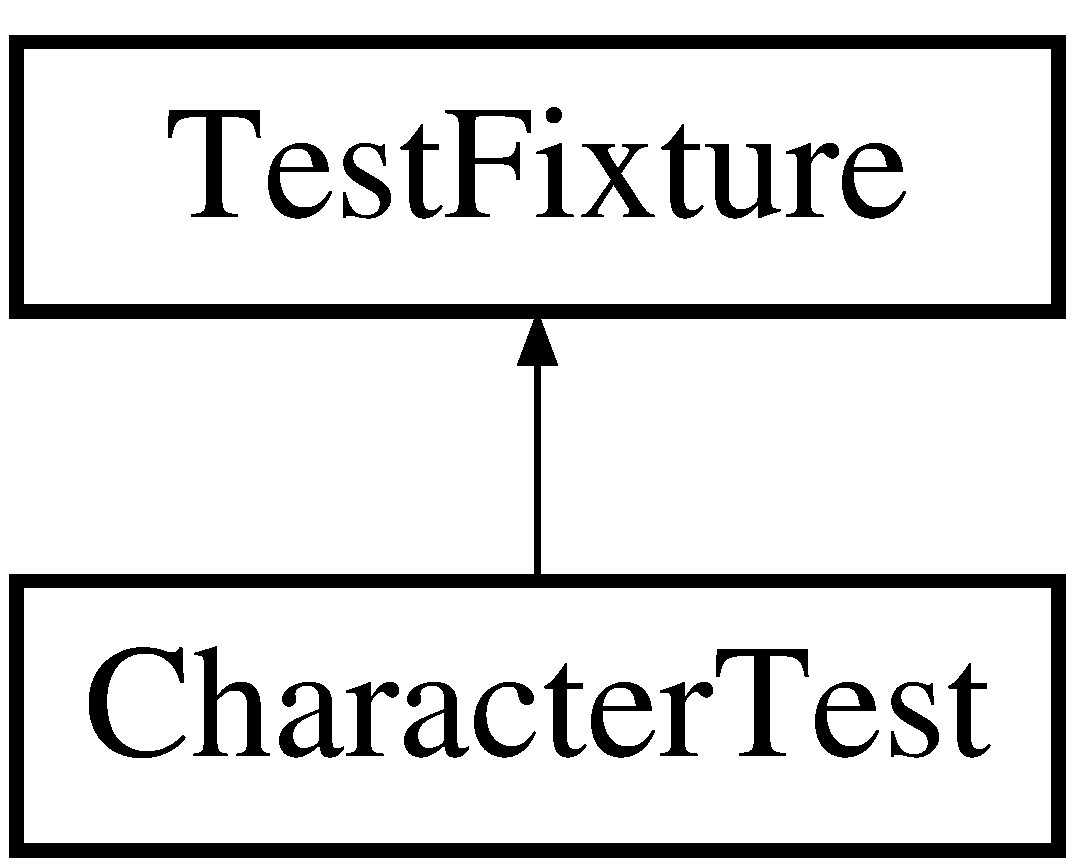
\includegraphics[height=2.000000cm]{class_character_test}
\end{center}
\end{figure}
\subsection*{Protected Member Functions}
\begin{DoxyCompactItemize}
\item 
void \hyperlink{class_character_test_a3b3fbf158ac905a62af5672e603a8c2d}{test\+Valid\+New\+Character} ()
\item 
void \hyperlink{class_character_test_a6685946b68744680e6a99989fed31581}{test\+Invalid\+New\+Character} ()
\item 
void \hyperlink{class_character_test_a43147b36c83f5a8aea5cd32ba00a3c54}{test\+Hit} ()
\end{DoxyCompactItemize}


\subsection{Detailed Description}
Test Class for the \hyperlink{class_character}{Character} class. 

\subsection{Member Function Documentation}
\hypertarget{class_character_test_a43147b36c83f5a8aea5cd32ba00a3c54}{}\index{Character\+Test@{Character\+Test}!test\+Hit@{test\+Hit}}
\index{test\+Hit@{test\+Hit}!Character\+Test@{Character\+Test}}
\subsubsection[{test\+Hit}]{\setlength{\rightskip}{0pt plus 5cm}void Character\+Test\+::test\+Hit (
\begin{DoxyParamCaption}
{}
\end{DoxyParamCaption}
)\hspace{0.3cm}{\ttfamily [protected]}}\label{class_character_test_a43147b36c83f5a8aea5cd32ba00a3c54}
test method to test the hit() method of the \hyperlink{class_map}{Map} class Test Case\+: a character that has been hit(x) should have its hit points reduced by x Tested item\+: \hyperlink{class_character_a2261aeb45173d9da1e8ff76a1db81928}{Character\+::hit()} \hypertarget{class_character_test_a6685946b68744680e6a99989fed31581}{}\index{Character\+Test@{Character\+Test}!test\+Invalid\+New\+Character@{test\+Invalid\+New\+Character}}
\index{test\+Invalid\+New\+Character@{test\+Invalid\+New\+Character}!Character\+Test@{Character\+Test}}
\subsubsection[{test\+Invalid\+New\+Character}]{\setlength{\rightskip}{0pt plus 5cm}void Character\+Test\+::test\+Invalid\+New\+Character (
\begin{DoxyParamCaption}
{}
\end{DoxyParamCaption}
)\hspace{0.3cm}{\ttfamily [protected]}}\label{class_character_test_a6685946b68744680e6a99989fed31581}
test method to test the validate\+New\+Character() method of the \hyperlink{class_character}{Character} class Test Case\+: an invalid newly created character should have any of its ability scores outside the \mbox{[}3-\/18\mbox{]} range Tested item\+: \hyperlink{class_character_adae2bb0e0bb6b8d010be6d1ac3b1fd5f}{Character\+::validate\+New\+Character()} \hypertarget{class_character_test_a3b3fbf158ac905a62af5672e603a8c2d}{}\index{Character\+Test@{Character\+Test}!test\+Valid\+New\+Character@{test\+Valid\+New\+Character}}
\index{test\+Valid\+New\+Character@{test\+Valid\+New\+Character}!Character\+Test@{Character\+Test}}
\subsubsection[{test\+Valid\+New\+Character}]{\setlength{\rightskip}{0pt plus 5cm}void Character\+Test\+::test\+Valid\+New\+Character (
\begin{DoxyParamCaption}
{}
\end{DoxyParamCaption}
)\hspace{0.3cm}{\ttfamily [protected]}}\label{class_character_test_a3b3fbf158ac905a62af5672e603a8c2d}
test method to test the validate\+New\+Character() method of the \hyperlink{class_character}{Character} class Test Case\+: a valid newly created character should have all its ability scores in the \mbox{[}3-\/18\mbox{]} range Tested item\+: \hyperlink{class_character_adae2bb0e0bb6b8d010be6d1ac3b1fd5f}{Character\+::validate\+New\+Character()} 

The documentation for this class was generated from the following file\+:\begin{DoxyCompactItemize}
\item 
\hyperlink{_character_test_8cpp}{Character\+Test.\+cpp}\end{DoxyCompactItemize}

\hypertarget{class_entity}{}\section{Entity Class Reference}
\label{class_entity}\index{Entity@{Entity}}


The documentation for this class was generated from the following file\+:\begin{DoxyCompactItemize}
\item 
entity.\+h\end{DoxyCompactItemize}

\hypertarget{class_map}{}\section{Map Class Reference}
\label{class_map}\index{Map@{Map}}
\subsection*{Public Member Functions}
\begin{DoxyCompactItemize}
\item 
\hypertarget{class_map_a8497952fd6e1f0584d868e6ceb97d42d}{}{\bfseries Map} (int width, int height)\label{class_map_a8497952fd6e1f0584d868e6ceb97d42d}

\item 
\hypertarget{class_map_a70adeb57203a2726cd5b2cbcf25628c5}{}\hyperlink{class_map_tile}{Map\+Tile} $\ast$ {\bfseries get\+Tile} (int x, int y)\label{class_map_a70adeb57203a2726cd5b2cbcf25628c5}

\item 
\hypertarget{class_map_a6163461180ebdb9acc0f2e9ecb768dd2}{}void {\bfseries set\+Tile} (\hyperlink{class_map_tile}{Map\+Tile} $\ast$tile, int x, int y)\label{class_map_a6163461180ebdb9acc0f2e9ecb768dd2}

\item 
\hypertarget{class_map_ac0a654733e7899a88c587e5c3cb7cc00}{}\hyperlink{class_entity}{Entity} $\ast$ {\bfseries get\+Entity} (int x, int y)\label{class_map_ac0a654733e7899a88c587e5c3cb7cc00}

\item 
\hypertarget{class_map_a12d3a76479f42bcac72d866a9f2cd343}{}\hyperlink{class_entity}{Entity} $\ast$ {\bfseries move\+Entity} (int x1, int y1, int x2, int y2)\label{class_map_a12d3a76479f42bcac72d866a9f2cd343}

\item 
\hypertarget{class_map_a7bc197a79eaab24f953721a7e1909cf0}{}\hyperlink{class_entity}{Entity} $\ast$ {\bfseries remove\+Entity} (int x, int y)\label{class_map_a7bc197a79eaab24f953721a7e1909cf0}

\item 
\hypertarget{class_map_acd22fe6b636278d8b26b5aca44d8897b}{}bool {\bfseries spawn\+Entity} (\hyperlink{class_entity}{Entity} $\ast$entity, int x, int y)\label{class_map_acd22fe6b636278d8b26b5aca44d8897b}

\item 
\hypertarget{class_map_afd34d12227676b3cebeed9f5fae2508f}{}int {\bfseries get\+Width} ()\label{class_map_afd34d12227676b3cebeed9f5fae2508f}

\item 
\hypertarget{class_map_a2b09c8875af2efb711fc3a022e70427d}{}int {\bfseries get\+Height} ()\label{class_map_a2b09c8875af2efb711fc3a022e70427d}

\end{DoxyCompactItemize}


The documentation for this class was generated from the following files\+:\begin{DoxyCompactItemize}
\item 
map.\+h\item 
map.\+cpp\end{DoxyCompactItemize}

\hypertarget{class_map_tile}{}\section{Map\+Tile Class Reference}
\label{class_map_tile}\index{Map\+Tile@{Map\+Tile}}
\subsection*{Public Member Functions}
\begin{DoxyCompactItemize}
\item 
\hypertarget{class_map_tile_a983d82363db202e5902fffe3c29c0a83}{}{\bfseries Map\+Tile} (int id)\label{class_map_tile_a983d82363db202e5902fffe3c29c0a83}

\item 
\hypertarget{class_map_tile_a9246c75eea35529c0a3ef88bb4536225}{}int {\bfseries get\+Id} ()\label{class_map_tile_a9246c75eea35529c0a3ef88bb4536225}

\item 
\hypertarget{class_map_tile_aa79a23c47ce28d247e1e97ed3a855101}{}bool {\bfseries get\+Walkable} ()\label{class_map_tile_aa79a23c47ce28d247e1e97ed3a855101}

\item 
\hypertarget{class_map_tile_a459e9254decb2500df2539ef7948689b}{}void {\bfseries set\+Walkable} (bool walkable)\label{class_map_tile_a459e9254decb2500df2539ef7948689b}

\item 
\hypertarget{class_map_tile_a06d963e18836fc0a6bce6fb55f487582}{}int {\bfseries get\+Movement\+Cost} ()\label{class_map_tile_a06d963e18836fc0a6bce6fb55f487582}

\end{DoxyCompactItemize}


The documentation for this class was generated from the following files\+:\begin{DoxyCompactItemize}
\item 
map\+\_\+tile.\+h\item 
map\+\_\+tile.\+cpp\end{DoxyCompactItemize}

\hypertarget{class_node}{}\section{Node Class Reference}
\label{class_node}\index{Node@{Node}}
\subsection*{Public Member Functions}
\begin{DoxyCompactItemize}
\item 
\hypertarget{class_node_a167857e82d68aecf75c74e0125ea3edb}{}{\bfseries Node} (int x, int y, int g, bool walkable)\label{class_node_a167857e82d68aecf75c74e0125ea3edb}

\item 
double \hyperlink{class_node_a5c4279782a1ae22a873e5b9d0c004124}{calculate\+Heuristic} (int, int)
\item 
double \hyperlink{class_node_a1e56091a513706cd12fe58ed5b9d7290}{get\+F\+Value} ()
\item 
double \hyperlink{class_node_a9c693e514c631c04ab72dc35ae5fedeb}{get\+Local\+F\+Value} ()
\item 
\hypertarget{class_node_aef58459d6e69d9e2eb7e6f154a4d8b62}{}bool {\bfseries operator==} (const \hyperlink{class_node}{Node} \&n1)\label{class_node_aef58459d6e69d9e2eb7e6f154a4d8b62}

\end{DoxyCompactItemize}
\subsection*{Public Attributes}
\begin{DoxyCompactItemize}
\item 
\hypertarget{class_node_afb5a7ac7536a9e09488bb685420cd78a}{}int {\bfseries h}\label{class_node_afb5a7ac7536a9e09488bb685420cd78a}

\item 
\hypertarget{class_node_a0b249888eacdec6c623ec8c58b230c48}{}int {\bfseries g}\label{class_node_a0b249888eacdec6c623ec8c58b230c48}

\item 
\hypertarget{class_node_a32fbe9e0f4fc9e9d1845ce808738d7ab}{}int {\bfseries f}\label{class_node_a32fbe9e0f4fc9e9d1845ce808738d7ab}

\item 
\hypertarget{class_node_aff1029a518bdc2651007b8856f958364}{}int {\bfseries x}\label{class_node_aff1029a518bdc2651007b8856f958364}

\item 
\hypertarget{class_node_aa3e5b5240023b4528ae85057b3324202}{}int {\bfseries y}\label{class_node_aa3e5b5240023b4528ae85057b3324202}

\item 
\hypertarget{class_node_a2fa5c14023fbc7849d0bb32e77bebf9d}{}bool {\bfseries walkable}\label{class_node_a2fa5c14023fbc7849d0bb32e77bebf9d}

\item 
\hypertarget{class_node_ad8184598cdea70e4bbdfd76f2b0f9e85}{}\hyperlink{class_node}{Node} $\ast$ {\bfseries parent}\label{class_node_ad8184598cdea70e4bbdfd76f2b0f9e85}

\end{DoxyCompactItemize}


\subsection{Member Function Documentation}
\hypertarget{class_node_a5c4279782a1ae22a873e5b9d0c004124}{}\index{Node@{Node}!calculate\+Heuristic@{calculate\+Heuristic}}
\index{calculate\+Heuristic@{calculate\+Heuristic}!Node@{Node}}
\subsubsection[{calculate\+Heuristic}]{\setlength{\rightskip}{0pt plus 5cm}double Node\+::calculate\+Heuristic (
\begin{DoxyParamCaption}
\item[{int}]{target\+X, }
\item[{int}]{target\+Y}
\end{DoxyParamCaption}
)}\label{class_node_a5c4279782a1ae22a873e5b9d0c004124}
calculate distance. using manhatan method \hypertarget{class_node_a1e56091a513706cd12fe58ed5b9d7290}{}\index{Node@{Node}!get\+F\+Value@{get\+F\+Value}}
\index{get\+F\+Value@{get\+F\+Value}!Node@{Node}}
\subsubsection[{get\+F\+Value}]{\setlength{\rightskip}{0pt plus 5cm}double Node\+::get\+F\+Value (
\begin{DoxyParamCaption}
{}
\end{DoxyParamCaption}
)}\label{class_node_a1e56091a513706cd12fe58ed5b9d7290}
Get F value with parent nodes. \hypertarget{class_node_a9c693e514c631c04ab72dc35ae5fedeb}{}\index{Node@{Node}!get\+Local\+F\+Value@{get\+Local\+F\+Value}}
\index{get\+Local\+F\+Value@{get\+Local\+F\+Value}!Node@{Node}}
\subsubsection[{get\+Local\+F\+Value}]{\setlength{\rightskip}{0pt plus 5cm}double Node\+::get\+Local\+F\+Value (
\begin{DoxyParamCaption}
{}
\end{DoxyParamCaption}
)}\label{class_node_a9c693e514c631c04ab72dc35ae5fedeb}
Get the local F value without parent nodes. 

The documentation for this class was generated from the following files\+:\begin{DoxyCompactItemize}
\item 
Pathfinder.\+h\item 
Pathfinder.\+cpp\end{DoxyCompactItemize}

\hypertarget{class_pathfinder}{}\section{Pathfinder Class Reference}
\label{class_pathfinder}\index{Pathfinder@{Pathfinder}}
\subsection*{Public Member Functions}
\begin{DoxyCompactItemize}
\item 
\hypertarget{class_pathfinder_ac8557a8750506a8409d3f633a931ceed}{}{\bfseries Pathfinder} (\hyperlink{class_map}{Map} $\ast$map, int, int)\label{class_pathfinder_ac8557a8750506a8409d3f633a931ceed}

\item 
void \hyperlink{class_pathfinder_a041c2195c3a5794e1ebdad07e8b91f53}{create\+Node\+Grid} ()
\item 
\hypertarget{class_pathfinder_abfdb0768b80340fc9a83cbb1026f7973}{}void {\bfseries refresh\+Heuristics} ()\label{class_pathfinder_abfdb0768b80340fc9a83cbb1026f7973}

\item 
\hypertarget{class_pathfinder_a040e7c1691958dc82a9559ec7f77f6d5}{}void {\bfseries set\+Destination} (int dx, int dy)\label{class_pathfinder_a040e7c1691958dc82a9559ec7f77f6d5}

\item 
std\+::vector$<$ \hyperlink{class_node}{Node} $\ast$ $>$ \hyperlink{class_pathfinder_a30bb66c6cee353d9807335eae326c6c0}{get\+Path} (int x1, int y1)
\item 
void \hyperlink{class_pathfinder_a06cfea5c03a992b177bff8eb3f53e41c}{print\+H\+Grid} ()
\end{DoxyCompactItemize}


\subsection{Member Function Documentation}
\hypertarget{class_pathfinder_a041c2195c3a5794e1ebdad07e8b91f53}{}\index{Pathfinder@{Pathfinder}!create\+Node\+Grid@{create\+Node\+Grid}}
\index{create\+Node\+Grid@{create\+Node\+Grid}!Pathfinder@{Pathfinder}}
\subsubsection[{create\+Node\+Grid}]{\setlength{\rightskip}{0pt plus 5cm}void Pathfinder\+::create\+Node\+Grid (
\begin{DoxyParamCaption}
{}
\end{DoxyParamCaption}
)}\label{class_pathfinder_a041c2195c3a5794e1ebdad07e8b91f53}
Create node grid from provided map. \hypertarget{class_pathfinder_a30bb66c6cee353d9807335eae326c6c0}{}\index{Pathfinder@{Pathfinder}!get\+Path@{get\+Path}}
\index{get\+Path@{get\+Path}!Pathfinder@{Pathfinder}}
\subsubsection[{get\+Path}]{\setlength{\rightskip}{0pt plus 5cm}std\+::vector$<$ {\bf Node} $\ast$ $>$ Pathfinder\+::get\+Path (
\begin{DoxyParamCaption}
\item[{int}]{x1, }
\item[{int}]{y1}
\end{DoxyParamCaption}
)}\label{class_pathfinder_a30bb66c6cee353d9807335eae326c6c0}
Get a path from x1, y1 to the destination \hypertarget{class_pathfinder_a06cfea5c03a992b177bff8eb3f53e41c}{}\index{Pathfinder@{Pathfinder}!print\+H\+Grid@{print\+H\+Grid}}
\index{print\+H\+Grid@{print\+H\+Grid}!Pathfinder@{Pathfinder}}
\subsubsection[{print\+H\+Grid}]{\setlength{\rightskip}{0pt plus 5cm}void Pathfinder\+::print\+H\+Grid (
\begin{DoxyParamCaption}
{}
\end{DoxyParamCaption}
)}\label{class_pathfinder_a06cfea5c03a992b177bff8eb3f53e41c}
Print grid of H values (distance) 

The documentation for this class was generated from the following files\+:\begin{DoxyCompactItemize}
\item 
Pathfinder.\+h\item 
Pathfinder.\+cpp\end{DoxyCompactItemize}

\chapter{File Documentation}
\hypertarget{_character_test_8cpp}{}\section{Character\+Test.\+cpp File Reference}
\label{_character_test_8cpp}\index{Character\+Test.\+cpp@{Character\+Test.\+cpp}}


Implementation file for the \hyperlink{class_character}{Character} Testing class.  


{\ttfamily \#include $<$cppunit/\+Test\+Case.\+h$>$}\\*
{\ttfamily \#include $<$cppunit/\+Test\+Fixture.\+h$>$}\\*
{\ttfamily \#include $<$cppunit/ui/text/\+Text\+Test\+Runner.\+h$>$}\\*
{\ttfamily \#include $<$cppunit/extensions/\+Helper\+Macros.\+h$>$}\\*
{\ttfamily \#include $<$cppunit/extensions/\+Test\+Factory\+Registry.\+h$>$}\\*
{\ttfamily \#include $<$cppunit/\+Test\+Result.\+h$>$}\\*
{\ttfamily \#include $<$cppunit/\+Test\+Result\+Collector.\+h$>$}\\*
{\ttfamily \#include $<$cppunit/\+Test\+Runner.\+h$>$}\\*
{\ttfamily \#include $<$cppunit/\+Brief\+Test\+Progress\+Listener.\+h$>$}\\*
{\ttfamily \#include $<$cppunit/\+Compiler\+Outputter.\+h$>$}\\*
{\ttfamily \#include $<$cppunit/\+Xml\+Outputter.\+h$>$}\\*
{\ttfamily \#include \char`\"{}character.\+h\char`\"{}}\\*
\subsection*{Classes}
\begin{DoxyCompactItemize}
\item 
class \hyperlink{class_character_test}{Character\+Test}
\begin{DoxyCompactList}\small\item\em Test Class for the \hyperlink{class_character}{Character} class. \end{DoxyCompactList}\end{DoxyCompactItemize}
\subsection*{Functions}
\begin{DoxyCompactItemize}
\item 
\hypertarget{_character_test_8cpp_a018bda66aa8778ad786c7ed9ed9229a6}{}\hyperlink{_character_test_8cpp_a018bda66aa8778ad786c7ed9ed9229a6}{C\+P\+P\+U\+N\+I\+T\+\_\+\+T\+E\+S\+T\+\_\+\+S\+U\+I\+T\+E\+\_\+\+R\+E\+G\+I\+S\+T\+R\+A\+T\+I\+O\+N} (\hyperlink{class_character_test}{Character\+Test})\label{_character_test_8cpp_a018bda66aa8778ad786c7ed9ed9229a6}

\begin{DoxyCompactList}\small\item\em test case registration \end{DoxyCompactList}\end{DoxyCompactItemize}


\subsection{Detailed Description}
Implementation file for the \hyperlink{class_character}{Character} Testing class. 


\hypertarget{_run_app_8cpp}{}\section{Run\+App.\+cpp File Reference}
\label{_run_app_8cpp}\index{Run\+App.\+cpp@{Run\+App.\+cpp}}


Driver file to create and execute the test suite.  


{\ttfamily \#include $<$cppunit/\+Compiler\+Outputter.\+h$>$}\\*
{\ttfamily \#include $<$cppunit/extensions/\+Test\+Factory\+Registry.\+h$>$}\\*
{\ttfamily \#include $<$cppunit/ui/text/\+Test\+Runner.\+h$>$}\\*
\subsection*{Functions}
\begin{DoxyCompactItemize}
\item 
int \hyperlink{_run_app_8cpp_a0ddf1224851353fc92bfbff6f499fa97}{main} (int argc, char $\ast$argv\mbox{[}$\,$\mbox{]})
\end{DoxyCompactItemize}


\subsection{Detailed Description}
Driver file to create and execute the test suite. 

Brief instruction on how to set Cpp\+Unit\+: from\+: http \+://www.comp.\+nus.\+edu.\+sg/$\sim$cs3215/tools/cppunit\+All.html

First, to install cpp\+Unit \+:


\begin{DoxyEnumerate}
\item Unpack the Cpp\+Unit archive (\href{https://sourceforge.net/projects/cppunit/files/cppunit/1.12.1/}{\tt https\+://sourceforge.\+net/projects/cppunit/files/cppunit/1.\+12.\+1/}) to a directory of your choice, in this example I assume it is D\+:.
\item Go to D\+:/cppunit-\/1.12.\+1/src and open the Cpp\+Unit\+Libraries.\+dsw in Visual Studio.
\item Select the cppunit project in the Solution Explorer and go to 'Project $>$ Properties $>$ Configuration Properties $>$ Librarian $>$ General. Put \char`\"{}\+Debug\textbackslash{}cppunit.\+lib\char`\"{} in the �\+Output File� textbox.
\item Right-\/click on the cppunit project in the Solution Explorer pane and choose Build.
\item After successful compilation, D\+:/cppunit-\/1.12.\+1/lib/cppunit.lib is produced which you then need to setup the Visual Studio Linker with (see below). 
\end{DoxyEnumerate}

\subsection{Function Documentation}
\hypertarget{_run_app_8cpp_a0ddf1224851353fc92bfbff6f499fa97}{}\index{Run\+App.\+cpp@{Run\+App.\+cpp}!main@{main}}
\index{main@{main}!Run\+App.\+cpp@{Run\+App.\+cpp}}
\subsubsection[{main}]{\setlength{\rightskip}{0pt plus 5cm}int main (
\begin{DoxyParamCaption}
\item[{int}]{argc, }
\item[{char $\ast$}]{argv\mbox{[}$\,$\mbox{]}}
\end{DoxyParamCaption}
)}\label{_run_app_8cpp_a0ddf1224851353fc92bfbff6f499fa97}
To setup a project from scratch for Compilation / Linking\+:


\begin{DoxyEnumerate}
\item Activate 'Project $>$ Properties $>$ C/\+C++ $>$ Code Generation $>$ Runtime Library $>$ Multi -\/ threaded Debug D\+L\+L'
\item Go to 'Project $>$ Properties $>$ C/\+C++ $>$ General'. Put \char`\"{}\+D\+:\textbackslash{}cppunit-\/1.\+12.\+1\textbackslash{}include\char`\"{} in the 'Additional Include Directories' text box.
\item Go to 'Project $>$ Properties $>$ Linker $>$ Input'. Put \char`\"{}\+D\+:\textbackslash{}cppunit-\/1.\+12.\+1\textbackslash{}lib\textbackslash{}cppunit.\+lib\char`\"{} in the 'Additional Dependences' text box.
\item Go to 'Project $>$ Properties $>$ Build Events $>$ Post-\/\+Build Event'. Put '\char`\"{}\$(\+Target\+Path)\char`\"{}' in the 'Command Line' textbox.\+Put 'Unit Tests...' in the 'Description' textbox. \hyperlink{_run_app_8cpp_a0ddf1224851353fc92bfbff6f499fa97}{main()} function. Entry point of the program It does the following\+:
\end{DoxyEnumerate}

Create a test suite object from the registry as populated by the code in the Test Classes
\begin{DoxyEnumerate}
\item Create a test runner that will execute all the tests in the registry
\item (optionally) sets an outputter that will output the results
\item Run the test cases. 
\end{DoxyEnumerate}
%--- End generated contents ---

% Index
\backmatter
\newpage
\phantomsection
\clearemptydoublepage
\addcontentsline{toc}{chapter}{Index}
\printindex

\end{document}
